\documentclass{article}
\usepackage{graphicx}
\usepackage[style=ieee]{biblatex} % Set the reference style to IEEE
\usepackage{xcolor}
\usepackage{hyperref}
\usepackage{titletoc}

\definecolor{companyBlue}{RGB}{30,42,86}
\hypersetup{
  colorlinks,
  linkcolor={blue}, % Set link color to blue
  urlcolor={purple} % Set URL color to red
}

\usepackage{array} % For customizing the table
\usepackage{booktabs} % For better quality horizontal lines
\usepackage{graphicx} % Package for including images
\usepackage{float}

% Define margins
\usepackage[margin=1in]{geometry}

\renewcommand{\contentsname}{\textcolor{companyBlue}{Table of Contents}}

\begin{document}

\begin{titlepage}
    \centering
    % University logo
    \includegraphics[width=0.24\textwidth]{logo.png}
    \par\vspace{2cm}

    % University name and course details
    {\Large \textbf{Data Analytics with PowerBI - APSCHE LTB3} \par}
    \vspace{0.5cm}
    {\large Seshadri Rao Gudlavalleru Engineering College \par}
    {\large Artificial Intelligence and Data Science \par}
    \vspace{3cm}

    % Lab and activity details
    {\large \textbf{Global Food Production Trends and Analysis} \par}
    {\large A Comprehensive Study from 1961 to 2023 Using Power BI \par}
    % {\large Specific topic \par}
    \vspace{3cm}

    % Team members
    {\large \textbf{Team} \par}
    \vspace{0.5cm}
    \begin{tabular}{ll}
    \textbf{Rohit Kavuluri} & \textbf{kavuluri.rohit@gmail.com} \\
    Basamsetti Purna Chandra Sekhar & purnachandrasekharb629@gmail.com \\
    Karra Prashanth & karraprashanth1911@gmail.com \\
    Adi Sandhya & adisandhya443@gmail.com \\
    \end{tabular}
    \par\vspace{3cm}

    % Date
    {\large March 04 2025 \par}
\end{titlepage}

\tableofcontents % Insert table of contents

\newpage % Page break to separate table of contents from document content

% Document content
\section{Introduction}\label{sec:example}
ABC Company undertook a comprehensive study of global food production trends from 1961 to 2023, leveraging Power BI for insightful visualizations. The analysis encompassed key agricultural commodities, revealing that total rice production amounted to 269 billion tonnes, while wheat production reached 282 billion tonnes. The study highlighted that tea production stood at 2 billion tonnes, with Africa emerging as the leading producer of green coffee. Additionally, the research underscored a steady rise in wheat, maize, and rice production over the years, with wheat showing the most significant increase. \\

The project also explored the production volumes of apples, avocados, bananas, and oranges by different regions, identifying Europe and Asia as significant contributors. Maize production demonstrated consistent growth, particularly from the late 1980s onward. The study further indicated that grapes had the highest total production among fruits at 43 billion tonnes, followed by apples, bananas, and oranges. This comprehensive analysis equips ABC Company with valuable insights to better understand global food production trends, aiding strategic decision-making in the agricultural sector. \\

\begin{itemize}

\item \textbf{Scenario 1} - Sum of Rice Production (tonnes)
This section prominently displays the total global rice production, amounting to 269 billion tonnes over the period from 1961 to 2023. It highlights the significant volume of rice produced, emphasizing its importance as a staple food crop worldwide. \\


\item \textbf{Scenario 2} - Sum of Wheat Production (tonnes)
Highlighting the global wheat production, this section shows a total of 282 billion tonnes produced between 1961 and 2023. This underscores wheat's crucial role in global food security and its widespread cultivation. \\

\item \textbf{Scenario 3} - Sum of Tea Production (tonnes)
This section shows a gauge chart illustrating the total tea production, amounting to 2 billion tonnes. The visual emphasizes the scale of tea production compared to other major crops. \\

\item \textbf{Scenario 4} - Sum of Coffee, Green Production (tonnes) by Entity
A bar chart depicting the distribution of green coffee production among various entities. Africa, Asia, and America are leading producers, reflecting regional contributions to global coffee supply. \\


\item \textbf{Scenario 5} - Sum of Wheat, Maize, and Rice Production (tonnes) by Year
An area chart showing the annual production trends of wheat, maize, and rice from 1961 to 2023. It highlights the growth trajectories and fluctuations of these essential crops over the years. \\

\item \textbf{Scenario 6} - Sum of Apples, Avocados, Bananas, and Oranges Production (tonnes) by Entity
This stacked bar chart illustrates the production volumes of apples, avocados, bananas, and oranges by different entities. It highlights the diverse contributions to global fruit production. \\

\item \textbf{Scenario 7} - Sum of Maize Production (tonnes) by Year
A donut chart depicting the yearly maize production distribution across different years. It shows how maize production has evolved, with specific years highlighted for their significant contributions. \\

\item \textbf{Scenario 8} - Sum of Grapes, Apples, Bananas, and Oranges Production (tonnes)
This bar chart compares the total production volumes of grapes (43 billion tonnes), apples (39 billion tonnes), bananas (32 billion tonnes), and oranges (26 billion tonnes). It provides a comparative view of the global production scales of these popular fruits.

\end{itemize}

\section{Technical Architecture}
\renewcommand{\tablename}{Figure}
\begin{figure}[H]
  \centering
  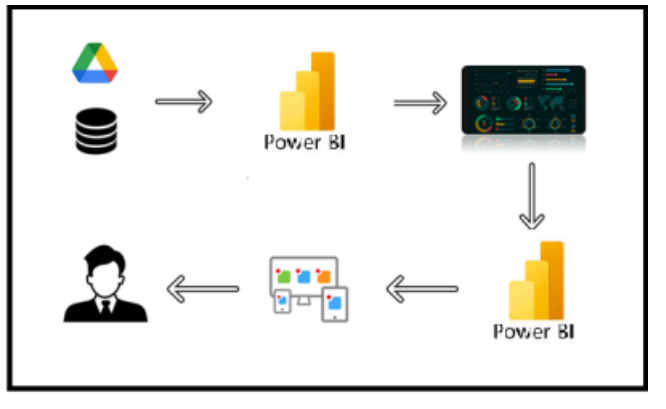
\includegraphics[width=0.7\textwidth]{project_flow.png}
  \caption{Flowchart of Project Architecture}
  \label{fig:project_flow}
\end{figure}

\section{Project Flow}
\begin{itemize}
    \item Data Collection
    \begin{itemize}
        \item Collect the dataset
        \item Connect Data with Power BI
    \end{itemize}
    \item Data Preparation
    \begin{itemize}
        \item Prepare the Data for Visualization
    \end{itemize}
    \item Data Visualizations
    \begin{itemize}
        \item Visualizations
    \end{itemize}
    \item Dashboard
    \begin{itemize}
        \item Responsive and Design of Dashboard
    \end{itemize}
    \item Report
    \begin{itemize}
        \item Report Creation
    \end{itemize}
    \item Performance Testing 
    \begin{itemize}
        \item Utilization of Data Filters
        \item No. of Calculation fields
        \item No of Visualizations/ Graphs 
    \end{itemize}
    \item Project Demonstration \& Documentation
    \begin{itemize}
        \item Record explanation Video for project end to end solution
        \item Project Documentation-Step by step project development procedure
    \end{itemize}
\end{itemize}

\section{Data Collection}
Data collection is the process of gathering and measuring information on variables of interest, in an established systematic fashion that enables one to answer stated research questions, test hypotheses, evaluate outcomes and generate insights from the data.

\subsection{Collect the dataset}
Please use the link to download the dataset: \textbf{\href{https://www.kaggle.com/datasets/rafsunahmad/world-food-production}{World Food Production}}


\subsubsection{Understand the data}
Data contains all the meta information regarding the columns described in the CSV files

Column Description of the Dataset:
\begin{itemize}
    \item Entity: Represents the country or region where the food production data is recorded.
    \item Code: A unique identifier or code for each entity (country or region).
    \item Year: The specific year for which the data is recorded, ranging from 1961 to 2023.
    \item Apples Production: The total annual production of apples measured in tonnes.
    \item Avocados Production: The total annual production of avocados measured in tonnes.
    \item Bananas Production: The total annual production of bananas measured in tonnes.
    \item Coffee green Production: The total annual production of green coffee measured in tonnes.
    \item Grapes Production: The total annual production of grapes measured in tonnes.
    \item Maize Production: The total annual production of maize measured in tonnes.
    \item Oranges Production: The total annual production of oranges measured in tonnes.
    \item Rice Production: The total annual production of rice measured in tonnes.
    \item Tea Production: The total annual production of tea measured in tonnes.
    \item Wheat Production: The total annual production of wheat measured in tonnes.
\end{itemize}

\subsection{Connect Data with PowerBI}
With Power BI, users can seamlessly connect to a wide range of data sources, including databases, cloud services, spreadsheets, and streaming data. This capability allows organizations to consolidate disparate data sources into a single, unified platform, breaking down data silos and enabling holistic analysis.

\section{Data Preparation}
Data Preparation is the process of transforming raw data into a clean and usable format, involving a systematic set of activities that enable effective analysis, modeling, and interpretation, ultimately facilitating accurate insights and informed decision-making.
\subsection{Prepare the Data for Visualization}
Preparing the data for visualization involves cleaning the data to remove irrelevant or missing data, transforming the data into a format that can be easily visualized, exploring the data to identify patterns and trends, filtering the data to focus on specific subsets of data, preparing the data for visualization software, and ensuring the data is accurate and complete. This process helps to make the data easily understandable and ready for creating visualizations to gain insights into the performance and efficiency. Since the data is already cleaned, we can move to visualization.
\subsubsection{Data Loading}
Data Loading is the process of transferring data from a source system to a target system, in a structured and systematic manner that enables efficient data analysis, reporting, and utilization within the target environment.
\subsubsection{Data Cleaning}
Data cleaning is the process of identifying and correcting (or removing) errors, inconsistencies, and inaccuracies within a dataset, in a systematic and methodical manner that ensures the data is accurate, complete, and reliable for analysis and decision-making.

\section{Data Visualization}
Data visualization is the process of creating graphical representations of data to help people understand and explore the information. The goal of data visualization is to make complex data sets more accessible, intuitive, and easier to interpret. By using visual elements such as charts, graphs, and maps, data visualizations can help people quickly identify patterns, trends, and outliers in the data.
\subsection{Visualizations}
\subsubsection{Sum of Rice Production}
\begin{figure}[H]
    \centering
    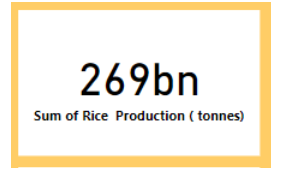
\includegraphics[width=0.4\textwidth]{rp.png}
    \caption{Sum of Rice Production}
    \label{fig:rp}
  \end{figure}
\subsubsection{Sum of Wheat Production}
\begin{figure}[H]
    \centering
    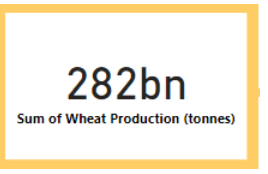
\includegraphics[width=0.4\textwidth]{wp.png}
    \caption{Sum of Wheat Production}
    \label{fig:wp}
  \end{figure}
\subsubsection{Sum of Tea Production}
\begin{figure}[H]
    \centering
    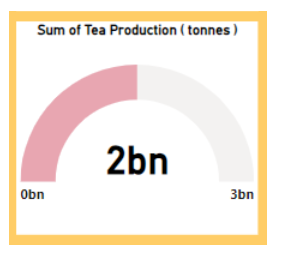
\includegraphics[width=0.4\textwidth]{tp.png}
    \caption{Sum of Tea Production}
    \label{fig:tp}
  \end{figure}
\subsubsection{Sum of Coffee, Green Production by Entity}
\begin{figure}[H]
    \centering
    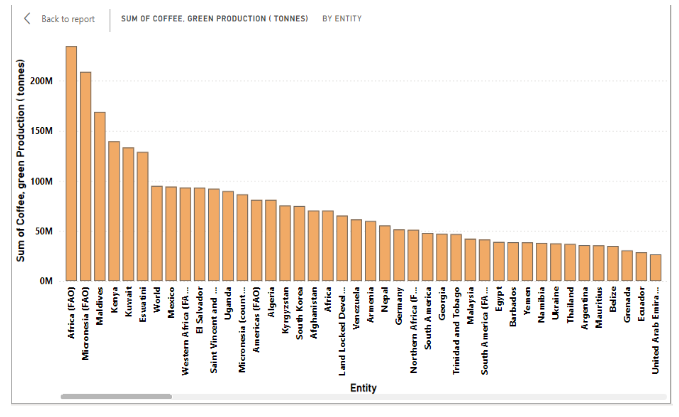
\includegraphics[width=0.4\textwidth]{cgp.png}
    \caption{Green Production by Entity}
    \label{fig:cgp}
  \end{figure}
\subsubsection{Sum of Wheat, Maize, and Rice Production by Year}
\begin{figure}[H]
    \centering
    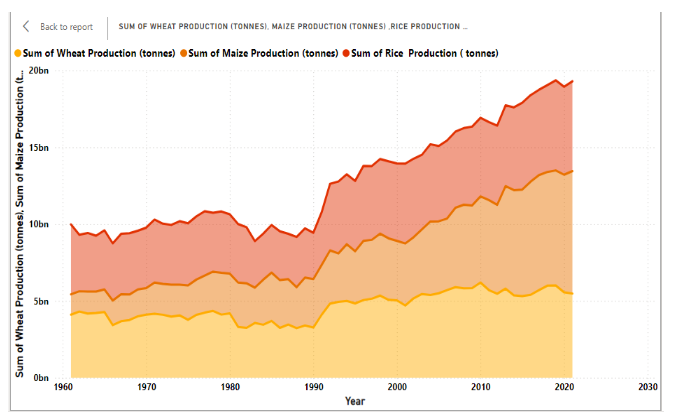
\includegraphics[width=0.4\textwidth]{wmr.png}
    \caption{Rice Production by Year}
    \label{fig:wmr}
  \end{figure}
\subsubsection{Sum of  Apples, Avocados, Bananas, and Oranges Production by Entity}
\begin{figure}[H]
    \centering
    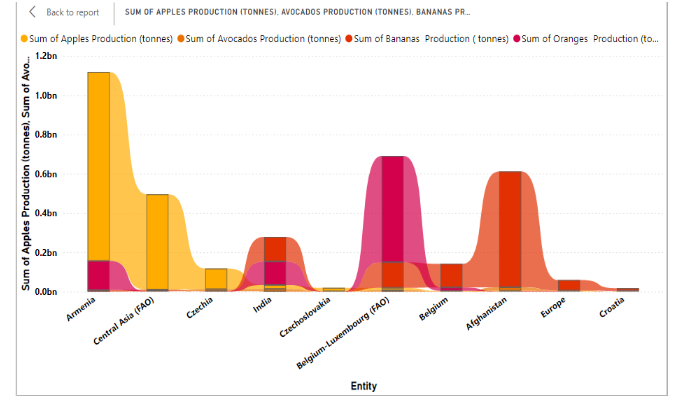
\includegraphics[width=0.4\textwidth]{aabo.png}
    \caption{Oranges Production by Entity}
    \label{fig:aabo}
  \end{figure}
\subsubsection{Sum of Maize Production by Year}
\begin{figure}[H]
    \centering
    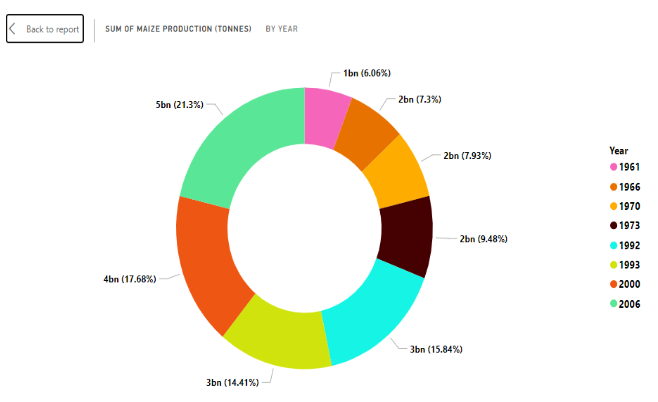
\includegraphics[width=0.4\textwidth]{mp.png}
    \caption{Maize Production by Year}
    \label{fig:mp}
  \end{figure}
\subsubsection{Sum of Grapes, Apples, Bananas, and Oranges Production}
\begin{figure}[H]
    \centering
    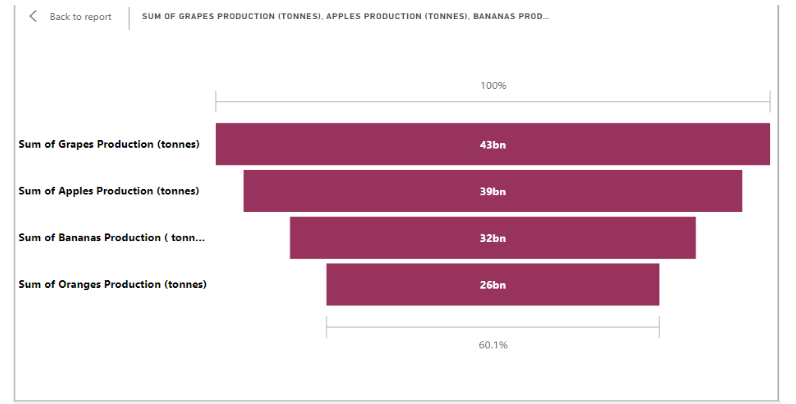
\includegraphics[width=0.4\textwidth]{gabo.png}
    \caption{Grapes, Apples, Bananas, and Oranges Production}
    \label{fig:gabo}
  \end{figure}

\section{Dashboard}
A dashboard is a graphical user interface (GUI) that displays information and data in an organized, easy-to-read format. Dashboards are often used to provide real-time monitoring and analysis of data and are typically designed for a specific purpose or use case. Dashboards can be used in a variety of settings, such as business, finance, manufacturing, healthcare, and many other industries. They can be used to track key performance indicators (KPIs), monitor performance metrics, and display data in the form of charts, graphs, and tables.
\subsection{Responsive and Design of Dashboard}
\begin{figure}[H]
    \centering
    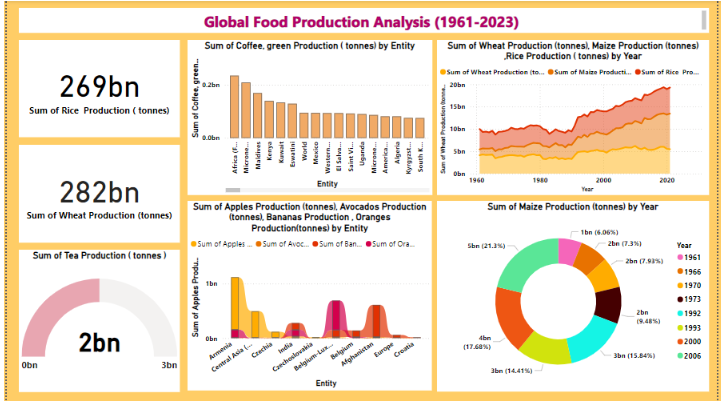
\includegraphics[width=1.0\textwidth]{dashboard.png}
    \caption{PowerBI Dashboard}
    \label{fig:dashboard}
  \end{figure}

\section{Report}
A report is a comprehensive document that provides a detailed and structured account of data analysis, findings, and insights. It is typically used for in-depth analysis, documentation, and communication of results. Reports are suitable for a diverse audience, including decision-makers, analysts, and stakeholders who need a comprehensive understanding of the data. 
\subsection{Design of Report}
Designing a report in Power BI involves connecting to data sources, creating visualizations like charts and graphs, customizing their appearance and interactivity, organizing them logically on the canvas, formatting elements for consistency and clarity, and optionally creating dashboards for a summarized view. Throughout the process, it's essential to consider the audience's needs and ensure the report effectively communicates insights from the data. Finally, iterate based on feedback to continually improve the report's design and usefulness.
\begin{figure}[H]
    \centering
    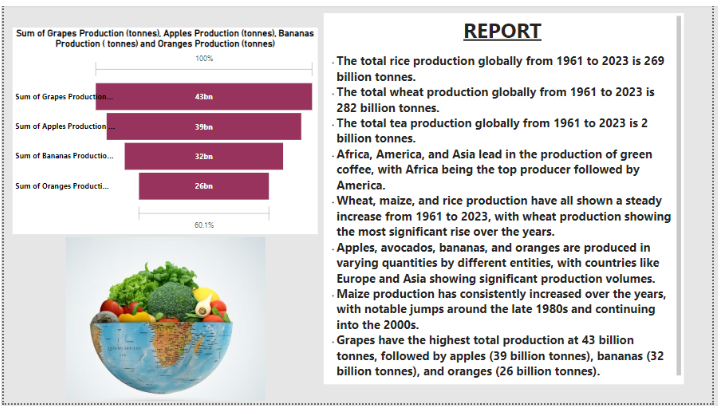
\includegraphics[width=0.8\textwidth]{report.png}
    \caption{PowerBI Report}
    \label{fig:report}
  \end{figure}

\section{Performance Testing}
Performance testing is the process of evaluating the speed, responsiveness, stability, and scalability of a system under varying workloads, in a controlled and systematic manner that enables one to identify bottlenecks, validate performance requirements, assess system behavior, and ensure optimal user experience.

\subsection{Amount of Data Loaded}
"Amount of Data Loaded" refers to the quantity or volume of data that has been imported, retrieved, or loaded into a system, software application, database, or any other data storage or processing environment. It's a measure of how much data has been successfully processed and made available for analysis, manipulation, or use within the system.
\begin{figure}[H]
    \centering
    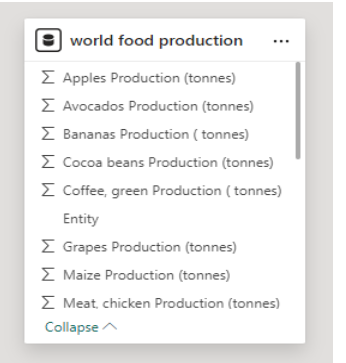
\includegraphics[width=0.3\textwidth]{data_loaded.png}
    \caption{Amount of Data Loaded}
    \label{fig:data_loaded}
  \end{figure}

\subsection{Utilization of Filters}
"Utilization of Filters" refers to the application or use of filters within a system, software application, or data processing pipeline to selectively extract, manipulate, or analyze data based on specified criteria or conditions.
\subsubsection{Selected “Country” as a Filter}
\begin{figure}[H]
    \centering
    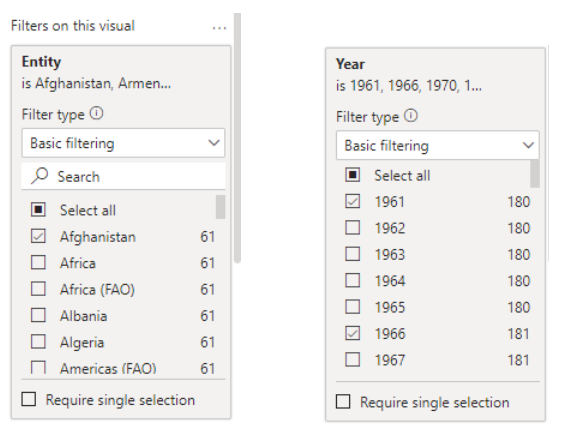
\includegraphics[width=0.4\textwidth]{country.png}
    \caption{Country Filter}
    \label{fig:country}
  \end{figure}
\subsubsection{No. of Visualizations/ Graphs}
\begin{itemize}
    \item Sum of Rice Production (tonnes)
    \item Sum of Wheat Production (tonnes)
    \item Sum of Tea Production (tonnes) 
    \item Sum of Coffee, Green Production (tonnes) by Entity
    \item Sum of Wheat Production (tonnes), Maize Production (tonnes), Rice Production (tonnes) by Year
    \item Sum of Apples, Avocados, Bananas, Oranges Production (tonnes) by Entity
    \item Sum of Maize Production (tonnes) by Year
    \item Sum of Grapes, Apples, Bananas, Oranges Production (tonnes)
\end{itemize}

\section{Project Documentation\& Demonstration}
\subsection{Project Documentation}
\textbf{\href{https://github.com/rohitprofc/global-food-production-trends-and-analysis}{Project's GitHub Repository Link}}
\subsection{Video Demonstration}
\textbf{\href{https://drive.google.com/drive/folders/1S8NCwMFRkYbBeIlY_46ocJlg5gv-J5vx?usp=sharing}{Drive Link to Video Demo}}

\end{document}